\chapter{Person Search Background}
Person search aims at finding a particular person from the gallery of pedestrian images. Because of its important applications in solving real-world problems, person search has received much attention in the past few years. Solving this problem is not easy. The complex variations of human poses, image resolutions, lighting conditions, camera viewpoints, occlusions, and background clutter make the person search more challenging. In Section~\ref{ps:reid}, we introduce existing person search categories. In Section~\ref{ps:method} and Section~\ref{ps:dataset}, we discuss some basic knowledge of person search, including the commonly used methods and datasets. Section~\ref{ps:evaluation} contains several evaluation methods.

\section{Person Search Categories}
\label{ps:reid}
Existing works of person search focus on automatically learning features with convolutional neural networks~\cite{li2014deepreid,ahmed2015improved} and learning distance metrics~\cite{prosser2010person,gray2008viewpoint,liao2015efficient}. 
Considering the type of input, person search can be categorized into image-based person search, video-based person search, and natural language based person search.

\textbf{Image-based Person Search.} Image-based person search, or person re-identification, usually uses \cite{koestinger2012large,farenzena2010person,bakone,pedagadi2013local,ma2012local,xiao2017joint,kviatkovsky2013color,xiao2016end} convolutional neural networks to learn features. Ahmed \etal \cite{ahmed2015improved} send a pair of images to a specifically designed CNN model with a binary classification loss for person re-identification. 
Ding \etal~\cite{ding2015deep} control the distances within the same person to be smaller than distances between different people using a triplet loss function.

\textbf{Video-based Person Search.} Video-based person search is an extension of image-based person search. The input is video sequences. Some people treat videos as a set of images and regard the video-based person search as multi-shot learning~\cite{hamdoun2008person,prosser2008multi,li2015locality}. Others extract the temporal information using RNN models~\cite{mclaughlin2016recurrent,zhousee,li2018diversity} or Optical Flow~\cite{mclaughlin2016recurrent,chung2017two}. In \cite{mclaughlin2016recurrent}, McLaughlin \etal introduce a RNN model to encode temporal information. Chung \etal~\cite{chung2017two} present a two stream convolutional neural network to learn spatial and temporal information separately.

\textbf{Natural Language based Person Search.} Image-based and video-based person search have major limitations in practice. They require at least one photo of the queried person being given. But in many criminal cases, there might be only verbal descriptions of the suspects' appearance available.
To close the gap, natural language descriptions are used as queries to search people. It does not require a person photo to be given as in those image-based or video-based query methods.

\section{Person Search Methods}
\label{ps:method}
\subsection{Identity Feature Learning}
Existing person search methods usually take the classification loss or triplet loss as the supervision to learn feature representations.
There are two types of classification settings as shown in Figure \ref{fig:loss} (a) and (b). The first type of methods treat the person search as a classification problem with the softmax loss function, \ie each person corresponds to a class in the training stage~\cite{xiao2016end,liao2015person,kumar2009attribute,xiao2016learning}. In the testing stage, we extract outputs before the last classification layer as person features and the similarity of two persons is evaluated by their feature distance. Even though this type of methods are easy to be implemented, there is a mismatch between the training and testing --- the training is a classification problem while the testing is a verification problem.

The second type of person search methods take two images as input and predict whether they contain the same person or not~\cite{ahmed2015improved,masi2016pose} (Figure \ref{fig:loss} (b)). The networks have a binary classification loss. We use the value of being class 1 as their matching score. However, methods with binary classification loss are time-consuming during the testing stage. To evaluate the performance of the proposed method, we need to construct $N^2$ image pairs and extract their features. $N$ is the number of testing samples. This may lead to longer evaluation time, especially on large-scale datasets.

For methods using triplet loss functions~\cite{cheng2016person,schroff2015facenet} (Figure \ref{fig:loss} (c)), their input consists of one anchor, one positive sample, and one negative sample. We train the model to minimize distances within the same person and maximize distances between different people. 

A new loss function, \eg Online Instance Matching, is proposed by Xiao \etal~\cite{xiao2017joint} recently. This loss function aims at solving the inefficiency of learning a large classification matrix in methods with the classification loss. The OIM is non-parametric. The gradients directly operate on the features without the transformation by a classifier matrix.

\begin{figure}[t]
\begin{center}
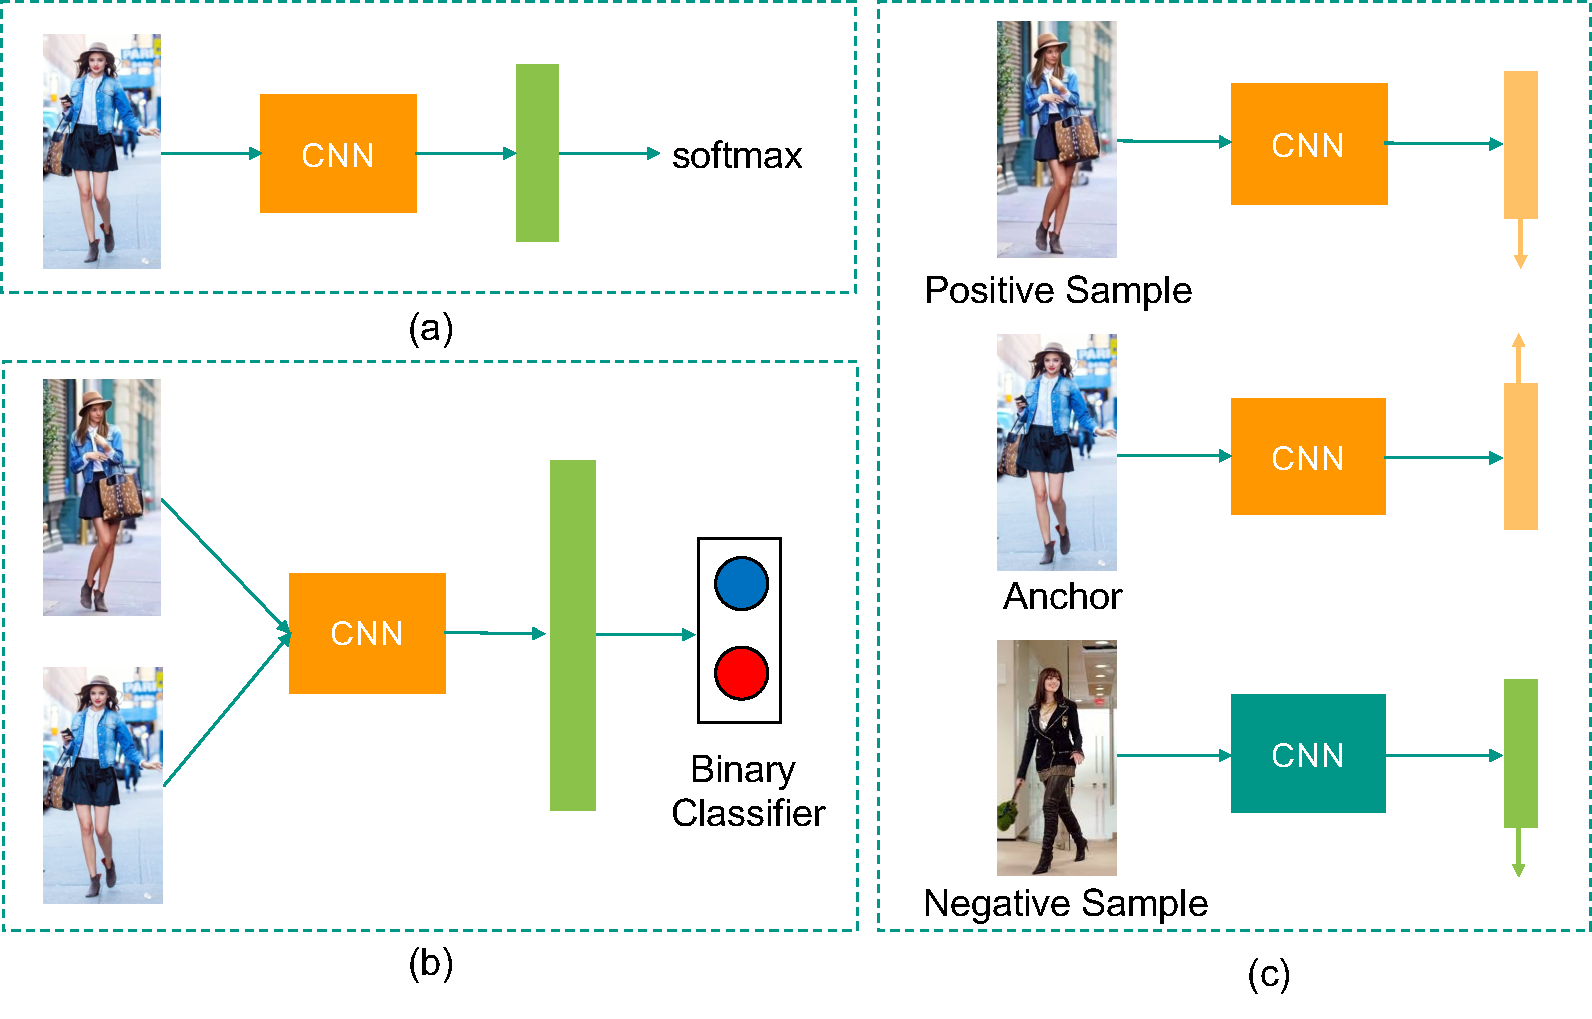
\includegraphics[width=1\linewidth]{figures/personsearch.pdf}
\caption{Identity feature learning using different loss functions.}
\label{fig:loss}
\end{center}
\end{figure}

\subsection{Feature Comparison}
Metric learning~\cite{davis2007information,weinberger2005distance,mcfee2010metric,koestinger2012large,liao2015person,zhang2016learning} is commonly used in early person search methods to compute the distance of two images. Suppose $x_1$ and $x_2$ are the feature representations of two persons, metric learning replaces conventional L2-distance by learning a distance function $d(x_1, x_2)$. Metric learning can be understood as learning a linear transformation on features, and thus it can be merged to deep learning models through fully-connected layers. The combination of a simple deep neural network and an L2-distance metric is a popular way to solve the person search problem.

Feature maps contain spatial information, but two feature maps are usually not well aligned. In the same position of two images, one could be a person's head and the other could be just the background. Comparing the distance of two feature maps is also an important strategy to evaluate their similarity. Li \etal~\cite{li2014deepreid} compute the correlation between the strips on two feature maps to estimate the similarity. In \cite{ahmed2015improved}, Ahmed \etal change the correlation from strips to local rectangle regions and improve the accuracy significantly. 

Bilinear pooling models also show impressive performance on fine-grained recognition tasks. They capture second-order statistics of convolutional features in a translationally invariant manner. Bilinear pooling methods have repeatedly shown to produce state-of-the-art results.
However, they are not widely adopted because their high dimensional features are impractical for subsequent analysis. Gao \etal~\cite{gao2016compact} propose two compact bilinear pooling methods to reduce the feature dimension. The compact bilinear pooling allows efficient end-to-end training.


%------------------------------------------------------------------------------------------
\begin{table}
\center
\begin{adjustbox}{max width=1\textwidth}
\begin{tabular}{lcccccc} 
\textsc{Dataset}        & Time      & \#ID       & \#Image        & \#Cameras  & Label     & Sequences\\
\hline
\textbf{VIPeR}~\cite{gray2007evaluating}          & 2007      & 632       &1,264 		    &2          & hand      & $\times$ \\ 
\textbf{QMUL iLIDS}~\cite{zheng2009associating}          & 2009      & 119     	&476            &2          & hand      & $\times$ \\ 
\textbf{GRID}~\cite{loy2009multi}        	& 2009      & 250       &1,275    	    &8          & hand      & $\times$ \\ 
\textbf{3DPeS}~\cite{baltieri20113dpes}                      & 2011      & 192       &1,011          &8          & hand      & $\times$ \\ 
\textbf{CUHK01}~\cite{li2012human}        	& 2012      & 971       &3,884    	    &2          & hand      & $\times$ \\ 
\textbf{CUHK02}~\cite{li2013locally}        	& 2013      & 1,816     &7,264    	    &10         & hand      & $\times$ \\ 
\textbf{CUHK03}~\cite{li2014deepreid} 	    & 2014      & 1,467     &13,164         &2          & hand/DPM  & $\times$ \\ 
\textbf{CUHK-SYSU}~\cite{xiaoli2017joint} 	    & 2016      & 8,432     &18,184         &-          & hand      & $\times$ \\ 
\textbf{Market-1501}~\cite{zheng2015scalable} 	& 2015      & 1,501     &32,668         &6          & hand/DPM  & $\times$ \\ 
\textbf{DukeMTMC}~\cite{zheng2017unlabeled}      & 2017      & 1,812     &36,441         &8          & hand      & $\times$ \\ 
\textbf{DukeMTMC4ReID}~\cite{zheng2017unlabeled} & 2017      & 1,852     &46,261         &8          & Doppia    & $\times$ \\ 
\hline
\textbf{PRID2011}~\cite{hirzer2011person} 	    & 2011      &934        &24,541         &2          & hand      & $\checkmark$ \\ 
\textbf{iLIDS-VID}~\cite{wang2014person} 	    & 2014      &300        &42,495         &2          & hand      & $\checkmark$ \\ 
\textbf{MARS}~\cite{zheng2016mars} 	        & 2016      &1,261      &1,191,003      &6          & DPM+GMMCP & $\checkmark$ \\ 
\hline
\end{tabular}
\end{adjustbox}
\caption{Statistics of some commonly used datasets for person search.}
\label{tab:dataset}
\end{table}
%------------------------------------------------------------------------------------------

\section{Datasets}
\label{ps:dataset}
A number of datasets have been released for research purpose. We list several the most commonly used image-based person search datasets and video-based datasets in Table \ref{tab:dataset}. VIPeR~\cite{gray2007evaluating} is the most popular dataset, containing 632 identities and 1,264 images. 10 random train/test splits are predefined for stable evaluations.
GRID~\cite{loy2009multi} is captured by 8 disjoint cameras in an underground station. Each identity has two images from different camera views. The image quality of this dataset is fairly poor.
QMUL iLIDS~\cite{zheng2009associating} and iLIDS-VID~\cite{wang2014person} are captured at the airport. They have scenarios with heavy occlusion and pose variance.
CUHK01~\cite{li2012human}, CUHK02~\cite{li2013locally}, and CUHK03~\cite{li2014deepreid} are collected from CUHK campus. In most existing datasets, the ground truth pedestrians are manually annotated. However, as the dataset size increases, CUHK03~\cite{li2014deepreid} and Market-1501~\cite{zheng2015scalable} introduce pedestrian detectors, such as DPM, to generate annotations. DukeMTMC4ReID~\cite{zheng2017unlabeled} uses the Doppia detector.
Samples in CUHK-SYSU~\cite{xiaoli2017joint} are mainly from street snaps and movies. Different from previous image-based datasets with cropped images, CUHK-SYSU provides whole scene images. This could trigger researchers to design methods that do pedestrian detection and person re-identification simultaneously. The problem setting of CUHK-SYSU is closer to real-world applications. 

PRID2011 \cite{hirzer2011person}, iLIDS-VID \cite{wang2014person}, and MARS \cite{zheng2016mars} are three video-based person search datasets. 
PRID2011 consists of person videos from two camera views. There are $385$ and $749$ identities in camera A and camera B respectively. Only the first $200$ people appear in both cameras. The sequence length ranges from 5 to 675 frames. 
iLIDS-VID contains 600 image sequences of 300 persons. For each person, we have two videos with the length of each video sequence varying from 23 to 192 frames. The average duration is 73 frames.
MARS dataset is the largest video-based person search benchmark with 1,261 identities and around 20,000 video sequences. They adopt DPM detector \cite{felzenszwalb2010object} and GMMCP tracker \cite{dehghan2015gmmcp} to extract the person sequence. Zheng \etal~\cite{zheng2016mars} set 6 cameras to collect data in the university campus. Each identity is captured by at least 2 cameras. This dataset also contains 3,248 distractor sequences. 

\section{Evaluation Metrics}
\label{ps:evaluation}
Cumulative Matching Characteristics (CMC) curve is usually used to evaluate person search algorithms. Taking the single-gallery-shot as an example, where there is only one matching identity for each query, the algorithm ranks all the gallery samples according to their similarities to the query. The CMC top-k accuracy is
\begin{equation}
  \mathrm{cmc}_k = \begin{cases}
    1 & \text{if the top-$k$ ranked gallery samples contains the correct matching,} \\
    0 & \text{otherwise}.
  \end{cases}
\end{equation}
The final CMC curve is the average value over all queries. This evaluation metric is acceptable to single-gallery-shot datasets. However, when it comes to the multi-gallery-shot setting, where each query has multiple ground truths existing in the gallery set, people define different criterions on different datasets.

Zheng \etal~\cite{zheng2015scalable} propose to use mean average precision (mAP) in the Market-1505 dataset. They compute the area under the precision-recall curve, \ie average precision (AP). The mAP is the mean value of AP.
In CUHK03, Li \etal randomly sample one instance for each gallery identity and compute the CMC curve. The process is repeated multiple times to generate the multi-gallery-shot CMC curve.